\appendix
%\gdef\thesection{Appendix \Alph{section}}

\fancychapter{Code Listings}

\begin{algorithm}[htb!]
\caption[Viterbi algorithm for multihit local alignment] {Pseudo-code of the Viterbi algorithm for multihit local alignment, with the superfluous transitions already removed.}
\label{code-viterbi}

\begin{algorithmic}

\State // Initialization:
\State	$  V^B (0) \gets log\ t_{N B}  $

\For{$i \gets 1 \textrm{ to } SequenceLength \ (L) $} 

	\State	 $ V^M_0(i)  \gets  V^D_0(i)  \gets  V^I_0(i)  \gets  V^E (i)  \gets  -infinity $

	\For{$j  \gets 1  \textrm{ to } ModelSize \ (MS) $} 

		\State	$ V^M_j(i) \gets log \frac{e_{Mj}(x_i) }{q_{xi}} + Max  
				\begin{cases}
					V^B \ (i-1)	    + log\ t_{B_{j-1} M_j} \\
					V^M_{j-1} (i-1) + log\ t_{M_{j-1} M_j}  \\
					V^I_{j-1} (i-1)  + log\ t_{I_{j-1} M_j}  \\
					V^D_{j-1} (i-1) + log\ t_{D_{j-1} M_j} 
				\end{cases} $


		\State	$ V^E_j (i) \gets  Max \begin{cases} 
						V^E_{j-1} (i) \\
						V^M_j(i) \\
						\end{cases} $
	   
		\State	$ V^I_j(i) \gets Max  
				\begin{cases}
					V^M_{j} (i-1) + log\ t_{M_{j} I_j}  \\
					V^I_{j} (i-1) + log\ t_{I_{j} I_j}
				\end{cases} $

		\State	$V^D_j(i) \gets Max \begin{cases}
					V^M_{j-1} (i) + log\ t_{M_{j-1} D_j}  \\
					V^D_{j-1} (i) + log\ t_{D_{j-1} D_j} 
				\end{cases} $ \\

	\EndFor

	
	\State // Updates of special states after the symbol's propagation through all the normal states:
	
	\State	$ V^E_{MS} (i) \gets Max \begin{cases} 
				 V^E_{MS} (i) \\
				 V^M_{MS} (i) \\
				\end{cases} $
	
	\State	$ V^J (i) \gets Max \begin{cases} 
				V^J (i) + log\ t_{J J}  \\
				V^E_{MS} (i) + log\ t_{E J} \\
				\end{cases} $	
					
	\State	$ V^C (i) \gets Max \begin{cases} 
				V^C (i) + log\ t_{C C}  \\
				V^E_{MS} (i) + log\ t_{E C} \\
				\end{cases} $
  
	\State	$ V^N (i) \gets V^N (i-1) + log\ t_{N N} $

	\State	$ V^B (i) \gets Max \begin{cases} 
				V^N (i) + log\ t_{N B}  \\
				V^J (i) + log\ t_{J B} \\
				\end{cases} $	
\EndFor
\end{algorithmic}
\end{algorithm}

\clearpage



\begin{algorithm}[htb!]
\caption[Forward algorithm for multihit local alignment] {Pseudo-code of the Forward algorithm for multihit local alignment, using the Interpolation/Lookup approach, and with the superflous transitions removed. The table $TabLog$ is pre-computed, as well as the logarithmic transition scores $log \; t_{X_j Y_i }$, and emission scores $log \frac{e_{Mj}(x_i) }{q_{xi}} $.}
\label{code-forward}
\begin{algorithmic}

\State // Initialization:
\State	$  F^B (0) \gets log\ t_{N B}  $

\For{$i \gets 1 \textrm{ to } SequenceLength \ (L) $} 

	\State	$ F^M_j(0) = F^D_j(0) = F^I_j(0) = F^E (i) = -infinity $

	\For{$j  \gets 1  \textrm{ to } ModelSize \ (MS) $} 
		\begin{align*}
		 F^M_j(i) = log \frac{e_{Mj}(x_i) }{q_{xi}} + TabLog \;\;  
				[ \ TabLog \ [ \;\; &log\ t_{M_{j-1}M_j} + \; (F^M_{j-1}(i-1)) \ , \\ 
						\;\; &log\ t_{I_{j-1} M_j}  + \; (F^I_{j-1}(i-1)) \ \ ] \ , \\
				TabLog \ [	\;\; &log\ t_{D_{j-1} M_j} + \; (F^D_{j-1}(i-1)) \ , 	\\
						\;\; &log\ t_{B_{j-1} M_j} + \; (F^B (i-1) \ ] \;\; ] 
		\end{align*}
		\begin{align*}
		&F^I_j(i)  \gets TabLog \;\; [ \;\; log\ t_{M_{j} I_j} + \; (F^M_{j}(i-1))  
					     	 + \;\; log\ t_{I_{j} I_j}  + \; (F^I_{j}(i-1))  \;\; ] 
		\\
		&F^D_j(i) \gets TabLog \;\; [ \;\; log\ t_{M_{j} D_j} + \; (F^M_{j-1}(i)) 
					    	  +\;\; log\ t_{M_{j} D_j} + \; (F^D_{j_1}(i))  \;\; ]
		\\
		& F^E_j (i) \gets TabLog \ \ [ F^E_{j-1} (i), TabLog \ [ \ F^M_j(i),  F^D_j(i) \ ] \ ] 
		\end{align*}

	\EndFor
	
	\State \\ Updates of special states after the symbol's propagation through all the normal states:

	\State	$ F^J (i) \gets TabLog \ [\ t_{J J} + F^J(i-1) \ ,  t_{E J} + F^E_{MS} (i) \ ] $

	\State	$ F^C (i) \gets TabLog\ [\ t_{C C} + F^C(i-1) \ ,  t_{E C} + F^E_{MS} (i) \ ] $

	\State	$ F^N (i) \gets log \ t_{N N} + F^N(i-1) $
	
	\State	$ F^B (i) \gets TabLog\ [\ t_{N B} + F^N(i) \ , t_{J B} + F^J(i) \ ] $

\EndFor

\end{algorithmic}
\end{algorithm}

\clearpage


\begin{algorithm}[htb!]
\caption[Initial inner loop code of COPS] {Initial inner loop code of COPS, based on Rognes Smith-Waterman implementation.}
\label{code-rognes}

\begin{algorithmic}
\\
\State $Initialize Mmx, Imx, Dmx to -Vinfinity$

\LeftComment Loop through the sequence symbols
\For {$i \gets 1 \textrm{ to } SequenceLength \ (L) $} 
		
	\State $LoadEmissionScores(e_{match}, i)$

	\State $ xmxE \gets mpv \gets dpv \gets ipv \gets sc \gets dcv \gets -Vinfinity $

	\LeftComment Loop through the model state-triplets
	\For {$i \gets 0 \textrm{ to } M-1 $} 

		\State $ Mnext \gets e_{match}(k) +  VMax
					\begin{cases}
						vB + t_{BM}(k)	\\
						Mpv + t_{MM}(k)	\\
						Ipv + t_{IM}(k)	\\
						Dpv + t_{DM}(k)	\\
					\end{cases} $ \\

		\State $ vE \gets VMax(vE, Mnext) $
		
		\LeftComment Pre-emptive load of M, D, I
		\State $ Dpv \gets Dmx(k) $
		\State $ Ipv  \gets Imx(k)  $
		\State $ Mpv \gets Mmx(k) $

		\LeftComment  Delayed stores of M and D
		\State $ Mmx(k) \gets Mnext $
		\State $ Dmx(k) \gets Dcv   $
		
		\LeftComment Calculate current I(k). $ e_{insert}$  always 0 in HMMER's unilocal mode
		\State $ Imx(k) \gets e_{insert} (k+1) + VMax
					\begin{cases}
						Mpv +  t_{MI}(k+1)	\\
						Ipv +  t_{II}(k+1)		\\
					\end{cases} $ \\

		\LeftComment Calculate next D, D(k+1)
		\State $ Dcv \gets VMax
					\begin{cases}
						Mnext +  t_{MD}(k+1)	\\
						Dcv +  t_{DD}(k+1)	\\
					\end{cases} $ 
	\EndFor
	
	\LeftComment Compute and update the special flanking states
	\State $ vJ  \gets VMAX(vJ + t_{JJ}, vE + t_{EJ})   $	\ \ \ \ \ \ // always 0 for HMMER's Unilocal mode
	\State $ vC \gets VMAX(vC + t_{CC}, vE + t_{EC}) $	\ \ \ \	// $t_{EC}$  is  0 
	\State $ vN \gets vN + t_{NN} $
	\State $ vB \gets VMAX(vN + t_{NM}, vJ + t_{JB})  $	\ \ \ \	// vJ is useless
\EndFor

\end{algorithmic}
\end{algorithm}

\clearpage


\begin{algorithm}[htb!]
\caption[Rognes code to load emission scores] {SSE code of Rognes method to load and arrange the Emission Scores }
\label{code-loading-rognes}

\begin{algorithmic}
\\
\For {$i \gets 1 \textrm{ to } M \textrm{ step }  4 $} 

	\LeftComment Load original scores
	\State	xmm[0] = \_mm\_load\_ps(EMscoreSeq[0]+k)
	\State	xmm[1] = \_mm\_load\_ps(EMscoreSeq[1]+k)
	\State	xmm[2] = \_mm\_load\_ps(EMscoreSeq[2]+k)
	\State xmm[3] = \_mm\_load\_ps(EMscoreSeq[3]+k)
	\LeftComment Interleave 32-bit wide
	\State xmm[4] = \_mm\_unpacklo\_ps(xmm[0], xmm[1])
	\State xmm[5] = \_mm\_unpackhi\_ps(xmm[0], xmm[1])
	\State xmm[6] = \_mm\_unpacklo\_ps(xmm[2], xmm[3])
	\State xmm[7] = \_mm\_unpackhi\_ps(xmm[2], xmm[3])
	\LeftComment Interleave 64-bit wide
	\State xmm[8]   = \_mm\_unpacklo\_pd(xmm[4], xmm[6])
	\State xmm[9]   = \_mm\_unpackhi\_pd(xmm[4], xmm[6])
	\State xmm[10] = \_mm\_unpacklo\_pd(xmm[5], xmm[7])
	\State xmm[11] = \_mm\_unpackhi\_pd(xmm[5], xmm[7])
	\LeftComment Store transposed values
	\State \_mm\_store\_si128(vEmsc+0, xmm[8])
	\State \_mm\_store\_si128(vEmsc+1, xmm[9])
	\State \_mm\_store\_si128(vEmsc+2, xmm[10])
	\State \_mm\_store\_si128(vEmsc+3, xmm[11])
	\State vEmsc = vEmsc + 4
\EndFor
\end{algorithmic}
\end{algorithm}
	
\clearpage




\begin{algorithm}[htb!]
\caption[Inline method code to load emission scores] {SSE code of the Inner loop with the Inline method to load and arrange the Emission Scores }
\label{code-loading-inline}

\begin{algorithmic}
\\
\For {$k \gets 1 \textrm{ to } M \textrm{ step }  4 $} 

	\LeftComment Load original scores
	\State	xmm[0] = \_mm\_load\_ps(EMscoreSeq[0]+k)
	\State	xmm[1] = \_mm\_load\_ps(EMscoreSeq[1]+k)
	\State	xmm[2] = \_mm\_load\_ps(EMscoreSeq[2]+k)
	\State xmm[3] = \_mm\_load\_ps(EMscoreSeq[3]+k)
	\LeftComment Interleave 32-bit wide
	\State xmm[4] = \_mm\_unpacklo\_ps(xmm[0], xmm[1])
	\State xmm[5] = \_mm\_unpackhi\_ps(xmm[0], xmm[1])
	\State xmm[6] = \_mm\_unpacklo\_ps(xmm[2], xmm[3])
	\State xmm[7] = \_mm\_unpackhi\_ps(xmm[2], xmm[3])
	\LeftComment Interleave 64-bit wide
	\State xmm[8]   = \_mm\_unpacklo\_pd(xmm[4], xmm[6])
	\State xmm[9]   = \_mm\_unpackhi\_pd(xmm[4], xmm[6])
	\State xmm[10] = \_mm\_unpacklo\_pd(xmm[5], xmm[7])
	\State xmm[11] = \_mm\_unpackhi\_pd(xmm[5], xmm[7])
	\LeftComment Macro with the inner loop code. Arguments: (model state index, xmm array index)
	\State COMPUTE\_TRIPLET\_STATE(k+0,8)
	\State	COMPUTE\_TRIPLET\_STATE(k+1,9)
	\State COMPUTE\_TRIPLET\_STATE(k+2,10)
	\State	COMPUTE\_TRIPLET\_STATE(k+3,11)
\EndFor
\end{algorithmic}
\end{algorithm}

\clearpage



\begin{algorithm}[h!]
\caption{Pseudo-code of the proposed COPS approach using SSE2 with 8x16-bit integers and saturated arithmetic. This is the final single-threaded version.}
\label{code-complete}

\begin{spacing}{1.08}
\begin{algorithmic}[1]
\item[]
\LeftComment  Loop through the partitions
\For {$p \gets 1 \textrm{ to } Npartitions $} 

	\State $ Initialize \;\; Mmx,\;\;Imx,\;\;Dmx\;\;to\;\; -\infty $

	\LeftComment Loop through the sequence symbols
	\For {$i \gets 1 \textrm{ to } SequenceLength \ (L) $} 
		
		\If { p = 0 }
			\LeftComment First partition, initialize all to $-\infty $
			\State $ xmxE \gets Mnext \gets Dcv \gets -\infty $
		\Else 
			\LeftComment Load data from previous partitions
			\State $xmxE \gets PxmxE(i) $
			\State $Dcv \;\;\; \gets PDcv(i) $
			\State $Mnext   \gets PMnext(i) $
		\EndIf

		\LeftComment Loop through the model state-triplets of the current partition
		\For {$k \gets 0 \textrm{ until } k = PartLength \textrm{ or } 
			 k + p \times PartLength > ModelLength \textrm{ step } 8 $} 
			\LeftComment Load original scores, xmm 0 to 8
			\State	$xmm[0] \gets LOAD16(EMscoreSeq[0]+k) $
			\State	$xmm[1] \gets LOAD32(EMscoreSeq[1]+k) $
			\State ...
			\LeftComment Interleave 16-bit wide, xmm 8 to 15
			\State $xmm[8] \gets UNPACK\_LOW16 (xmm[0], xmm[1]) $
			\State $xmm[9] \gets UNPACK\_HIGH16(xmm[0], xmm[1]) $
			\State ...
			\LeftComment Interleave 32-bit wide, xmm 16 to 23
			\State $xmm[16] \gets UNPACK\_LOW32 (xmm[8], xmm[10]) $
			\State $xmm[17] \gets UNPACK\_HIGH32(xmm[8], xmm[10]) $
			\State ...
			\LeftComment Interleave 64-bit wide, xmm 24 to 31
			\State $xmm[24] \gets UNPACK\_LOW64 (xmm[16], xmm[18) $
			\State $xmm[25] \gets UNPACK\_HIGH64(xmm[16], xmm[18]) $
			\State ...
			\LeftComment Macro with the inner loop code, xmm 24 to 31
			\State $ COMPUTE\_STATE\_TRIPLET(k+0,24) $
			\State	$ COMPUTE\_STATE\_TRIPLET(k+1,25) $
			\State ...
		\EndFor
	
		\LeftComment Compute and update the special flanking states
		\If { $ k + p \times PartLength < ModelLength $ }
			\LeftComment Not the last partiton, store data for next partition
			\State $ PxmxE(i) \gets xmxE $
			\State $ PDcv(i) \gets Dcv $
			\State $ PMnext(i) \gets Mnext $
		\Else 
			\LeftComment Final partition, update the definitive pseudo-states
			\State $ xmxC \gets VMAX16(xmxC, xmxE) $
		\EndIf
	\EndFor
\EndFor

\State \Return $ Undiscretize(VMAX16(xmxC,  t\_{CT})) $
\end{algorithmic}
\end{spacing}
\end{algorithm}

\clearpage



\begin{algorithm}[h!]
\caption{Core inner loop code, used in the macro COMPUTE\_STATE\_TRIPLET(Model State index, Emission Score index). Variable $k$ is the State index}
\label{code-compute}

\begin{algorithmic}[1]
\item[]
\LeftComment Use M value partially computed in last iteration
\State $ Mnext \gets VMAX16
			\begin{cases}
				Mnext \\						
				xmxB + t_{BM}(k)	\\
				xmx[EMindex])
			\end{cases} $ 
\item[]
\item[]
\State $ xmxE \gets VMAX16(vE, Mnext) $		
\item[]
\LeftComment Load scores from last column
\State $ Dpv \gets Dmx(k) $
\State $ Ipv  \gets Imx(k)  $
\State $ Mpv \gets Mmx(k) $
\item[]
\LeftComment Compute and store scores of this column
\State $ Mmx(k) \gets Mnext $
\State $ Dmx(k) \gets Dcv   $

\State $ Imx(k) \gets VMAX16
			\begin{cases}
				Mpv +  t_{MI}(k+1)	\\
				Ipv +  t_{II}(k+1)	\\
			\end{cases} $ 
\item[]
\item[]
\LeftComment Preempetive computation of next-column D score
\State $ Dcv \gets VMAX16
			\begin{cases}
				Mnext +  t_{MD}(k+1)	\\
				Dcv +  t_{DD}(k+1)	\\
			\end{cases} $ 
\item[]
\item[]
\LeftComment Partially compute M score for next column
\State $ Mnext \gets VMAX16
			\begin{cases}
				Mpv + t_{MM}(k)	\\
				Ipv  + t_{IM}(k)	\\
				Dpv + t_{DM}(k)	\\
			\end{cases} $ 
\item[]
\end{algorithmic}
\end{algorithm}
			
\clearpage





\fancychapter{Results of the Wave-Front Multi-threading}

\myparagraph{Wave-Front Multi-threading Results on AMD Opteron Bulldozer} 

\begin{figure}[h!]
    \begin{minipage}{0.48\linewidth}
		\centering
		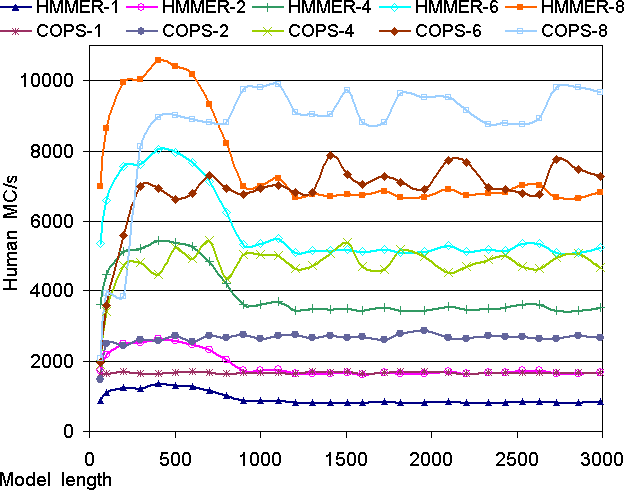
\includegraphics[scale=0.46]{graphics/threads-aleph-runtimes-human.png}
		\caption[Speeds of the multi-threaded COPS and HMMER, AMD Opteron, Human] 
		{Benchmark speeds of multi-threaded COPS and HMMER, on an AMD Opteron Bulldozer, for the Human genome}
		\label{threads-aleph-runtimes-human}
    \end{minipage}
    \hspace{0.04\linewidth}
    \begin{minipage}{0.48\linewidth}
		\centering
		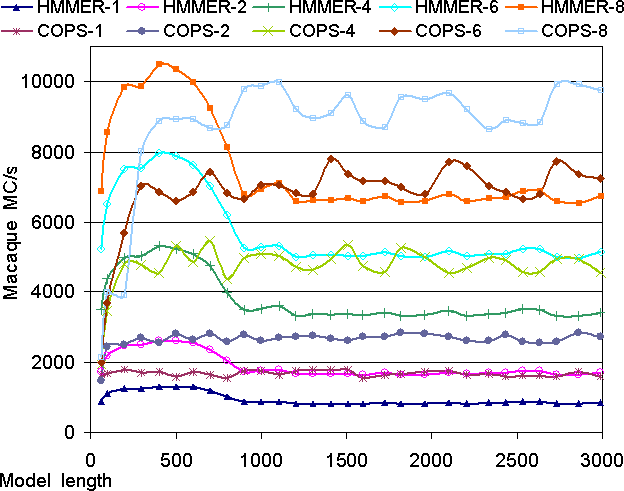
\includegraphics[scale=0.46]{graphics/threads-aleph-runtimes-macaque.png}
		\caption[Speeds of the multi-threaded COPS and HMMER, AMD Opteron, Macaque] 
		{Benchmark speeds of multi-threaded COPS and HMMER, on an AMD Opteron Bulldozer, for the Macaque genome.}
		\label{threads-aleph-runtimes-macaque}
    \end{minipage}
\end{figure} 

\begin{figure}[h!]
    \begin{minipage}{0.48\linewidth}
		\centering
		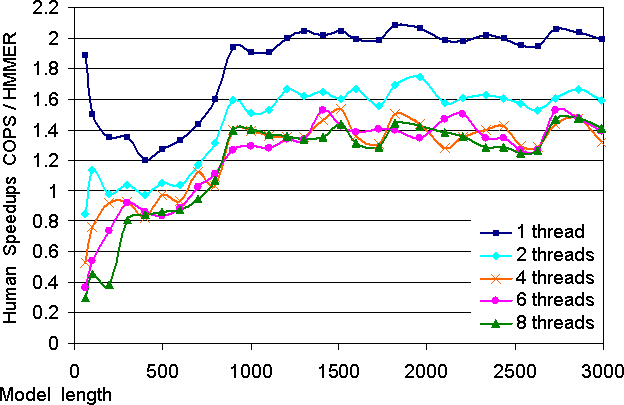
\includegraphics[scale=0.46]{graphics/threads-aleph-speedups-human.png}
		\caption[Speedups of the multi-threaded COPS vs HMMER, AMD Opteron, Human] 
		{Benchmark speedups of multi-threaded COPS vs HMMER, on an AMD Opteron Bulldozer, for the Human genome}
		\label{threads-aleph-speedups-human}
    \end{minipage}
    \hspace{0.04\linewidth}
    \begin{minipage}{0.48\linewidth}
		\centering
		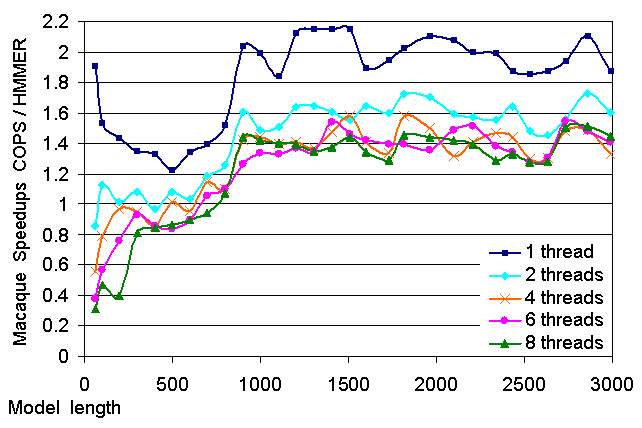
\includegraphics[scale=0.46]{graphics/threads-aleph-speedups-macaque.png}
		\caption[Speedups of the multi-threaded COPS vs HMMER, AMD Opteron, Macaque] 
		{Benchmark speedups of multi-threaded COPS vs HMMER, on an AMD Opteron Bulldozer, for the Macaque genome.}
		\label{threads-aleph-speedups-macaque}
    \end{minipage}
\end{figure} 

\clearpage

\myparagraph{Wave-Front Multi-threading Results on Intel Xeon Nehalem} 

\begin{figure}[h!]
    \begin{minipage}{0.48\linewidth}
		\centering
		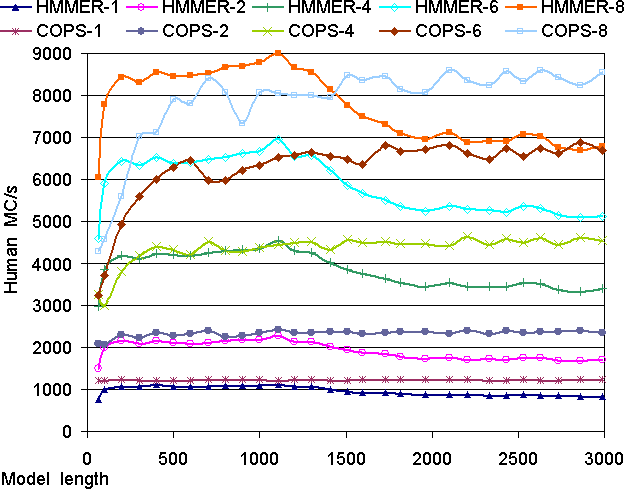
\includegraphics[scale=0.46]{graphics/threads-tags-runtimes-human.png}
		\caption[Speeds of the multi-threaded COPS and HMMER, Intel Xeon, Human] 
		{Benchmark speeds of multi-threaded COPS and HMMER, on an Intel Xeon Nehalem, for the Human genome}
		\label{threads-tags-runtimes-human}
    \end{minipage}
    \hspace{0.04\linewidth}
    \begin{minipage}{0.48\linewidth}
		\centering
		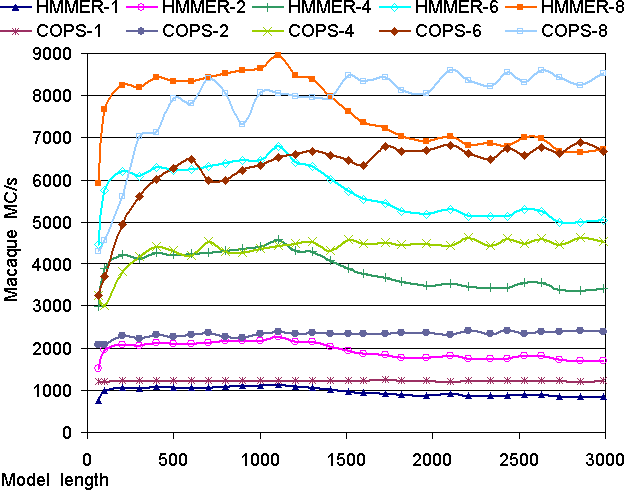
\includegraphics[scale=0.46]{graphics/threads-tags-runtimes-macaque.png}
		\caption[Speeds of the multi-threaded COPS and HMMER, Intel Xeon, Macaque] 
		{Benchmark speeds of multi-threaded COPS and HMMER, on an Intel Xeon Nehalem, for the Macaque genome.}
		\label{threads-tags-runtimes-macaque}
    \end{minipage}
\end{figure} 

\begin{figure}[h!]
    \begin{minipage}{0.48\linewidth}
		\centering
		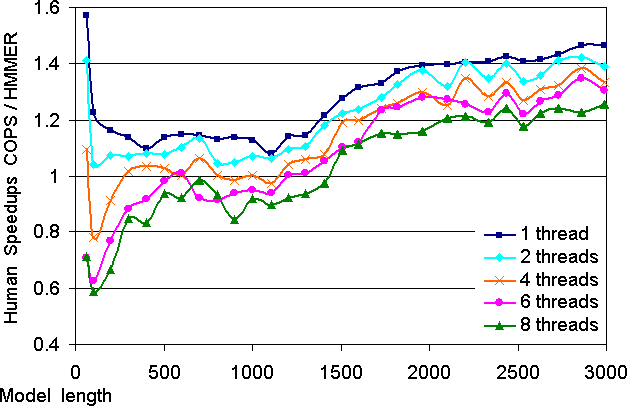
\includegraphics[scale=0.46]{graphics/threads-tags-speedups-human.png}
		\caption[Speedups of the multi-threaded COPS vs HMMER, Intel Xeon, Human] 
		{Benchmark speedups of multi-threaded COPS vs HMMER, on an Intel Xeon Nehalem, for the Human genome}
		\label{threads-tags-speedups-human}
    \end{minipage}
    \hspace{0.04\linewidth}
    \begin{minipage}{0.48\linewidth}
		\centering
		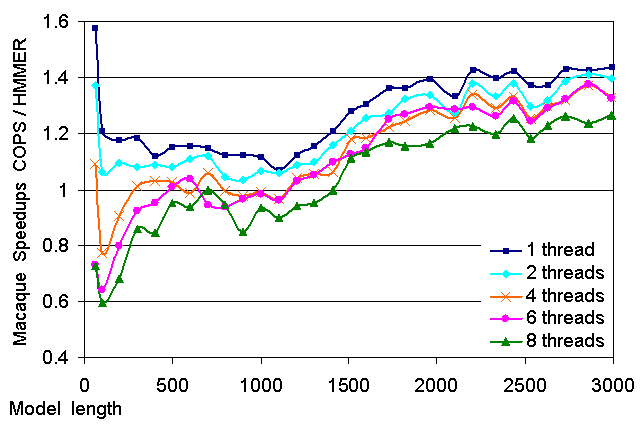
\includegraphics[scale=0.46]{graphics/threads-tags-speedups-macaque.png}
		\caption[Speedups of the multi-threaded COPS vs HMMER, Intel Xeon, Macaque] 
		{Benchmark speedups of multi-threaded COPS vs HMMER, on an Intel Xeon Nehalem, for the Macaque genome.}
		\label{threads-tags-speedups-macaque}
    \end{minipage}
\end{figure} 

\clearpage

\myparagraph{Wave-Front Multi-threading Results on Intel Core i7 Sandy Bridge} 

\begin{figure}[h!]
    \begin{minipage}{0.48\linewidth}
		\centering
		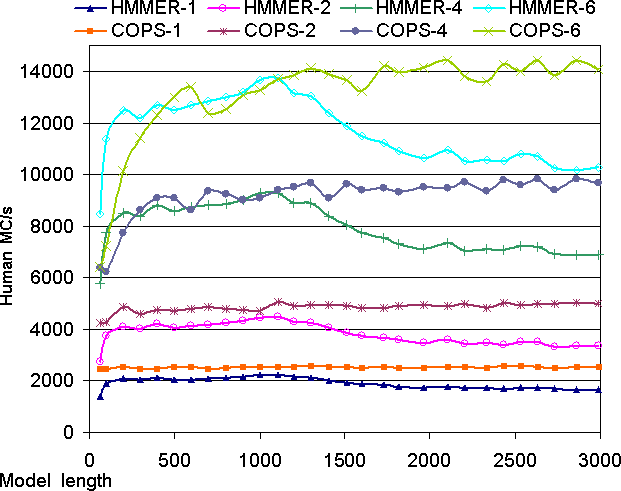
\includegraphics[scale=0.46]{graphics/threads-larissa-runtimes-human.png}
		\caption[Speeds of the multi-threaded COPS and HMMER, Intel Core i7, Human] 
		{Benchmark speeds of multi-threaded COPS and HMMER, on an Intel Core i7 Sandy Bridge, for the Human genome}
		\label{threads-larissa-runtimes-human}
    \end{minipage}
    \hspace{0.04\linewidth}
    \begin{minipage}{0.48\linewidth}
		\centering
		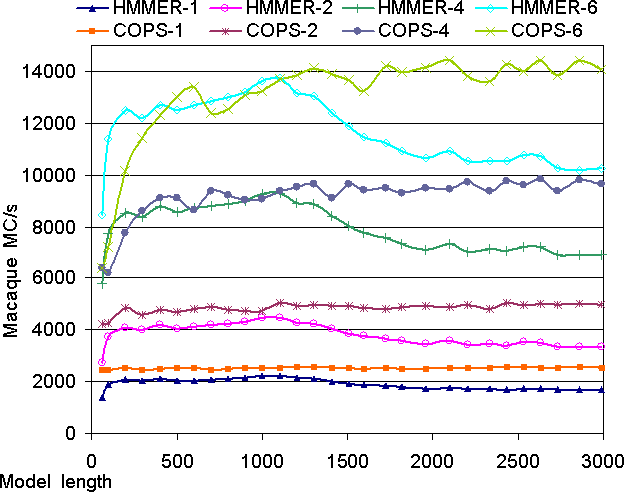
\includegraphics[scale=0.46]{graphics/threads-larissa-runtimes-macaque.png}
		\caption[Speeds of the multi-threaded COPS and HMMER, Intel Core i7, Macaque] 
		{Benchmark speeds of multi-threaded COPS and HMMER, on an Intel Core i7 Sandy Bridge, for the Macaque genome.}
		\label{threads-larissa-runtimes-macaque}
    \end{minipage}
\end{figure} 

\begin{figure}[h!]
    \begin{minipage}{0.48\linewidth}
		\centering
		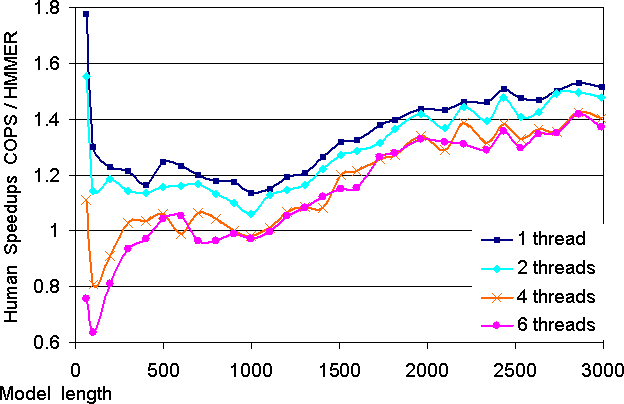
\includegraphics[scale=0.46]{graphics/threads-larissa-speedups-human.png}
		\caption[Speedups of the multi-threaded COPS vs HMMER, Intel Core i7, Human] 
		{Benchmark speedups of multi-threaded COPS vs HMMER, on an Intel Core i7 Sandy Bridge, for the Human genome}
		\label{threads-larissa-speedups-human}
    \end{minipage}
    \hspace{0.04\linewidth}
    \begin{minipage}{0.48\linewidth}
		\centering
		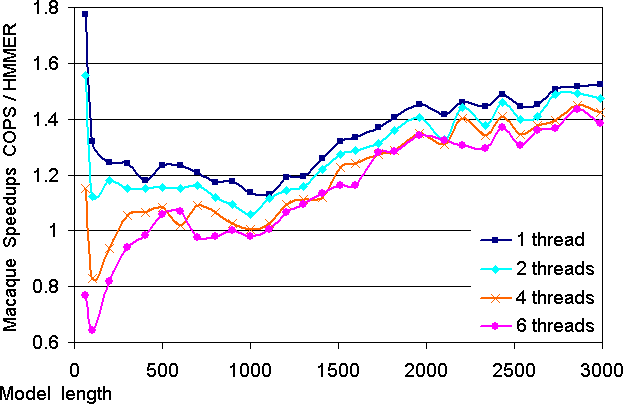
\includegraphics[scale=0.46]{graphics/threads-larissa-speedups-macaque.png}
		\caption[Speedups of the multi-threaded COPS vs HMMER, Intel Core i7, Macaque] 
		{Benchmark speedups of multi-threaded COPS vs HMMER, on an Intel Core i7 Sandy Bridge, for the Macaque genome.}
		\label{threads-larissa-speedups-macaque}
    \end{minipage}
\end{figure} 

